\documentclass[10pt]{article}
\usepackage[utf8]{inputenc}
\usepackage{graphicx}
\usepackage{tabularx}
\usepackage{titling}
\usepackage[a4paper,left=25mm,right=25mm,top=25mm,bottom=25mm,headsep=10mm,headheight=24pt]{geometry}
\usepackage{fancyhdr}
\usepackage{lastpage}
\usepackage[figure]{totalcount}
\usepackage{makecell}
\usepackage[T1]{fontenc}
\usepackage{tgadventor}

\renewcommand{\familydefault}{\sfdefault}
\renewcommand{\baselinestretch}{1.25} 

\newcommand{\thesubtitle}{High Level Design Document}
\newcommand{\theversion}{v1.0}
\newcommand{\thewebsite}{spaceymonk.github.io}
\renewcommand*\contentsname{Table of Contents}
\title{MentorHub}
\author{Berktuğ Kaan Özkan}


\pagestyle{fancy}
\fancyhf{}
\fancyhfoffset[L]{1cm} % left extra length
\fancyhfoffset[R]{1cm} % right extra length
\rhead{\today}
\chead{ \textbf{\thesubtitle{}} \\ \theversion{} }
\lhead{ \thetitle{} }
\lfoot{ \textit{\the\year{} \copyright{} \thewebsite{}} }
\rfoot{ \thepage{} of \pageref{LastPage} }
\cfoot{}


\begin{document} 


\begin{titlepage}
\begin{center}
    \vspace*{1cm}
    
    {\Huge
    
    \textbf{\thetitle}
    
    \vspace{1.0cm}
    
    \textbf{\thesubtitle{}}}
        
    \vspace{1.5cm}

    {\LARGE
    \theauthor

    \vfill
        
    Version \theversion{}
    
    \vspace{0.5cm}
    
    \today{}}
    
    \vspace{0.5cm}
   \end{center}
\end{titlepage}


\tableofcontents
\iftotalfigures
    \newpage
    \listoffigures
\fi
\newpage


\section{Introduction} \label{introduction}


\subsection{Purpose} \label{purpose}
This software design document describes the architecture, implemented features
and system design of MentorHub application. \textit{MentorHub  is a platform
application which enables it's users to find or to become mentors about their expertise.}


\subsection{Scope} \label{scope}
This document outlines the high level functional design of MentorHub application.
It highlights/refers the high level flows/use cases in design of components, along
with the rationale for the same. It serves as an input to the low level design 
documents that would further elaborate on the application design.


\subsection{Reference Material} \label{reference_material}
\begin{enumerate}
    \item OBSS Company 2021 Java Summer Internship Directive (July 2021 v1.0)
\end{enumerate} 


\subsection{Definitions and Acronyms} \label{definitions_and_acronyms}
\begin{table}[h]
    \centering
    \begin{tabularx}{\textwidth}{|l|X|}
    \hline
    \textbf{Term} & \textbf{Definition} \\ \hline
    LDAP    &  Lightweight Directory Access Protocol    \\ \hline
    SMTP & Simple Mail Transfer Protocol \\ \hline
    API & Application Programming Interface \\ \hline
    JVM & Java Virtual Machine \\ \hline
    Docker & Docker is a set of platform as a service products that use OS-level virtualization to deliver software in packages called containers. \\ \hline
    \end{tabularx}
    \label{tab:terms}
\end{table}
\newpage


\section{System Overview} \label{system_overview}

\subsection{Product Perspective} \label{product_perspective}
In a broader sense, users in the system will be able to provide mentoring support to
other users about their expertise.

Experts, mentoring on the subject of expertise will provide mentoring support to the
person concerned, based on the mentoring request received after the application is
approved. The users can see their former applications with additional information 
such as status and Admin's note if they got rejected. After Admin answered to request,
an email will be sent to the user.

When the mentoring process begins, the mentor and the user (mentee) will come together,
either online or offline, to determine the phases of the relevant process together with
their due dates and enter them into the system. After entering the system, they will
start the process and will be able to manage the phase changes over the system. In a
mentoring process, only one phase can be active at any time t.

The mentor or mentee will finish the relevant phase through a button in the system when
each phase is finished. After finishing the phase a review button will be activated.
After clicking this button, a display containing a text field where users can write their
comment and a field where users can give a score between 1 and 5 will open on the screen.
After the phase is over, the person who has not closed the phase will be able to read the
evaluation made by the person who closed it and make an evaluation comment himself/herself
and give a score.

The system will be notify the mentor and the mentee of a phase, 1 hour before the end
of the active phase, by sending email.

A user can become a mentor or a mentee at the same time.


\subsection{Tools Used} \label{tools_used}
The detailed list will be presented in the next sections. In general, the following tools
have used:
\begin{itemize}
    \item Maven based Java Spring Boot Framework for the main entry point.
    \item Thymeleaf, HTML, CSS and JavaScript used for the end-user interface design.
    For additional support following libraries used,
    \begin{itemize}
        \item JQuery Library for enhancing interactivity.
        \item Bootstrap 5 Library for the industrial standards in visuals.
    \end{itemize}
    \item Actual persistent data is stored in NoSQL database, MongoDB.
    \item Search engine selected as Elasticsearch due to advanced search capabilities
    (i.e. full--text search).
    \item The connection between MongoDB and Elasticsearch is established with Monstache.
    \item In order to quick and stable distribution of the software Docker containers used.
\end{itemize}


\subsection{Assumptions} \label{assumptions}
This project is designed with an educational mindset. Therefore, the resulting program
should not be used in real applications, as is. Main concern is the lack of security,
because the feature implementation was the first goal. Also in order to run application
with email support an SMTP server needs to be configured.


\section{System Architecture} \label{system_architecture}


\subsection{User Requirements} \label{user_requirements}


\subsubsection{Functional Requirements} \label{functional_requirements}
\begin{enumerate}

\item \textbf{Users and Roles}

There will be two type of user profiles: Admins and Users. 

\textit{There is no administrative interface to manage user profiles. User definitions
will be obtained from Google Authentication and LDAP server.}


\item \textbf{Subject Definitions}

Admins will be able to add new subjects, edit and remove existing subjects from the system.


\item \textbf{Creating Mentorship Requests}

Users can apply to become mentor by selecting the subjects which expertise in and writing
about themselves.


\item \textbf{Displaying Former Mentorship Requests}

Users can see their former applications with additional information such as date, status and 
Admin’s note if they got rejected.


\item \textbf{Accepting and Declining the Mentorship Requests}

The application requests will be presented to Admins after they logged in. They can either
accept or decline waiting requests made by Users.

If they rejected an request, they can write a comment about the refusal.


\item \textbf{Mentor Searching}

Users can search among accepted mentors in real time by entering a search text or by selecting
relevant subjects from a filter. Mentorship creation will be done by selecting a mentor from
this page.

\textit{One mentee can only work with one mentor under the same major subject. However, 
one mentor can only work with 2 mentees at the same time.}


\item \textbf{Phase Planning}

After mentorship creation, users will create/edit/remove phases of that mentoring process by
specifying a name, an end date and end time.

\textit{This process can be called as long as the mentoring process hasn't begun.}


\item \textbf{Displaying Mentorship Details}

Each user will see their mentoring processes after selecting a mentor. They can start the
process from here and see the comments/ratings about a specific phase.


\item \textbf{Phase Reviews}

After each phase completion, both mentor and mentee will write a short comment and give a
rating between 1 to 5 stars about finished phase.


\item \textbf{Email Reminder}

An email will be sent in following situations:
\begin{itemize}
    \item If there is less than one hour to end of an active phase, an email will be sent 
    to both mentor and mentee.
    \item After Admin answered to request, an email will be sent to the user.
\end{itemize}

\textit{MailHog container used for testing email reminder feature.}

\end{enumerate}


\subsubsection{Non--Functional Requirements} \label{nonfunctional_requirements}
\begin{enumerate}

\item \textbf{Authentication and Authorization}

Users can securely log into the system and access appropriate information based on their
role and account. Authentication of users should be done in following ways:
\begin{itemize}
    \item Login by LDAP
    \item Login by Google Authentication
\end{itemize}


\item \textbf{Security}

In order to access a page/resource users must be logged in. Logged in users can only access
and view/change their own data, they cannot view/change others.


\item \textbf{Performance}

Application should be fast enough to handle at least 1K users and 10K of mentorship process.
It should be stable while performing.


\item \textbf{Accessibility}

Application should be designed with flexible, user--friendly UI/UX and it should be
responsive (i.e. work on mobile phones and tablet).


\item \textbf{User interface}

The user interface is a very simple plain layout with little to no graphics. It will display
information very clearly for the user and will primarily output information to the user
through HTML pages formed with Thymeleaf framework. Administrative screens are use mainly
for input through text fields in HTML pages. Screen shots have been provided to demonstrate
the user and administrative interface, see section \ref{process_flow}.


\item \textbf{Error Handling}

Should errors be encountered, an explanation will be displayed as to what went wrong.

\textit{An error will be defined as anything that falls outside the normal and intended usage.}


\item \textbf{Maintainability}

Very little maintenance should be required for this setup. An initial configuration will be
the only system required interaction after system is put together. For example, defining
user roles.


\item \textbf{Portability}

This system should have the ability that, once it is together, the entire system should be
able to be moved to any location, easily.  Since the system deployed as Docker containers
it is easy to do so.

\end{enumerate}
\newpage


\subsubsection{Process Flow} \label{process_flow}
According to user requirements as defined in section \ref{user_requirements}, application
workflow and interfaces can be seen from the below figure \ref{fig:views}.

\begin{figure}[ht!]
    \centering
    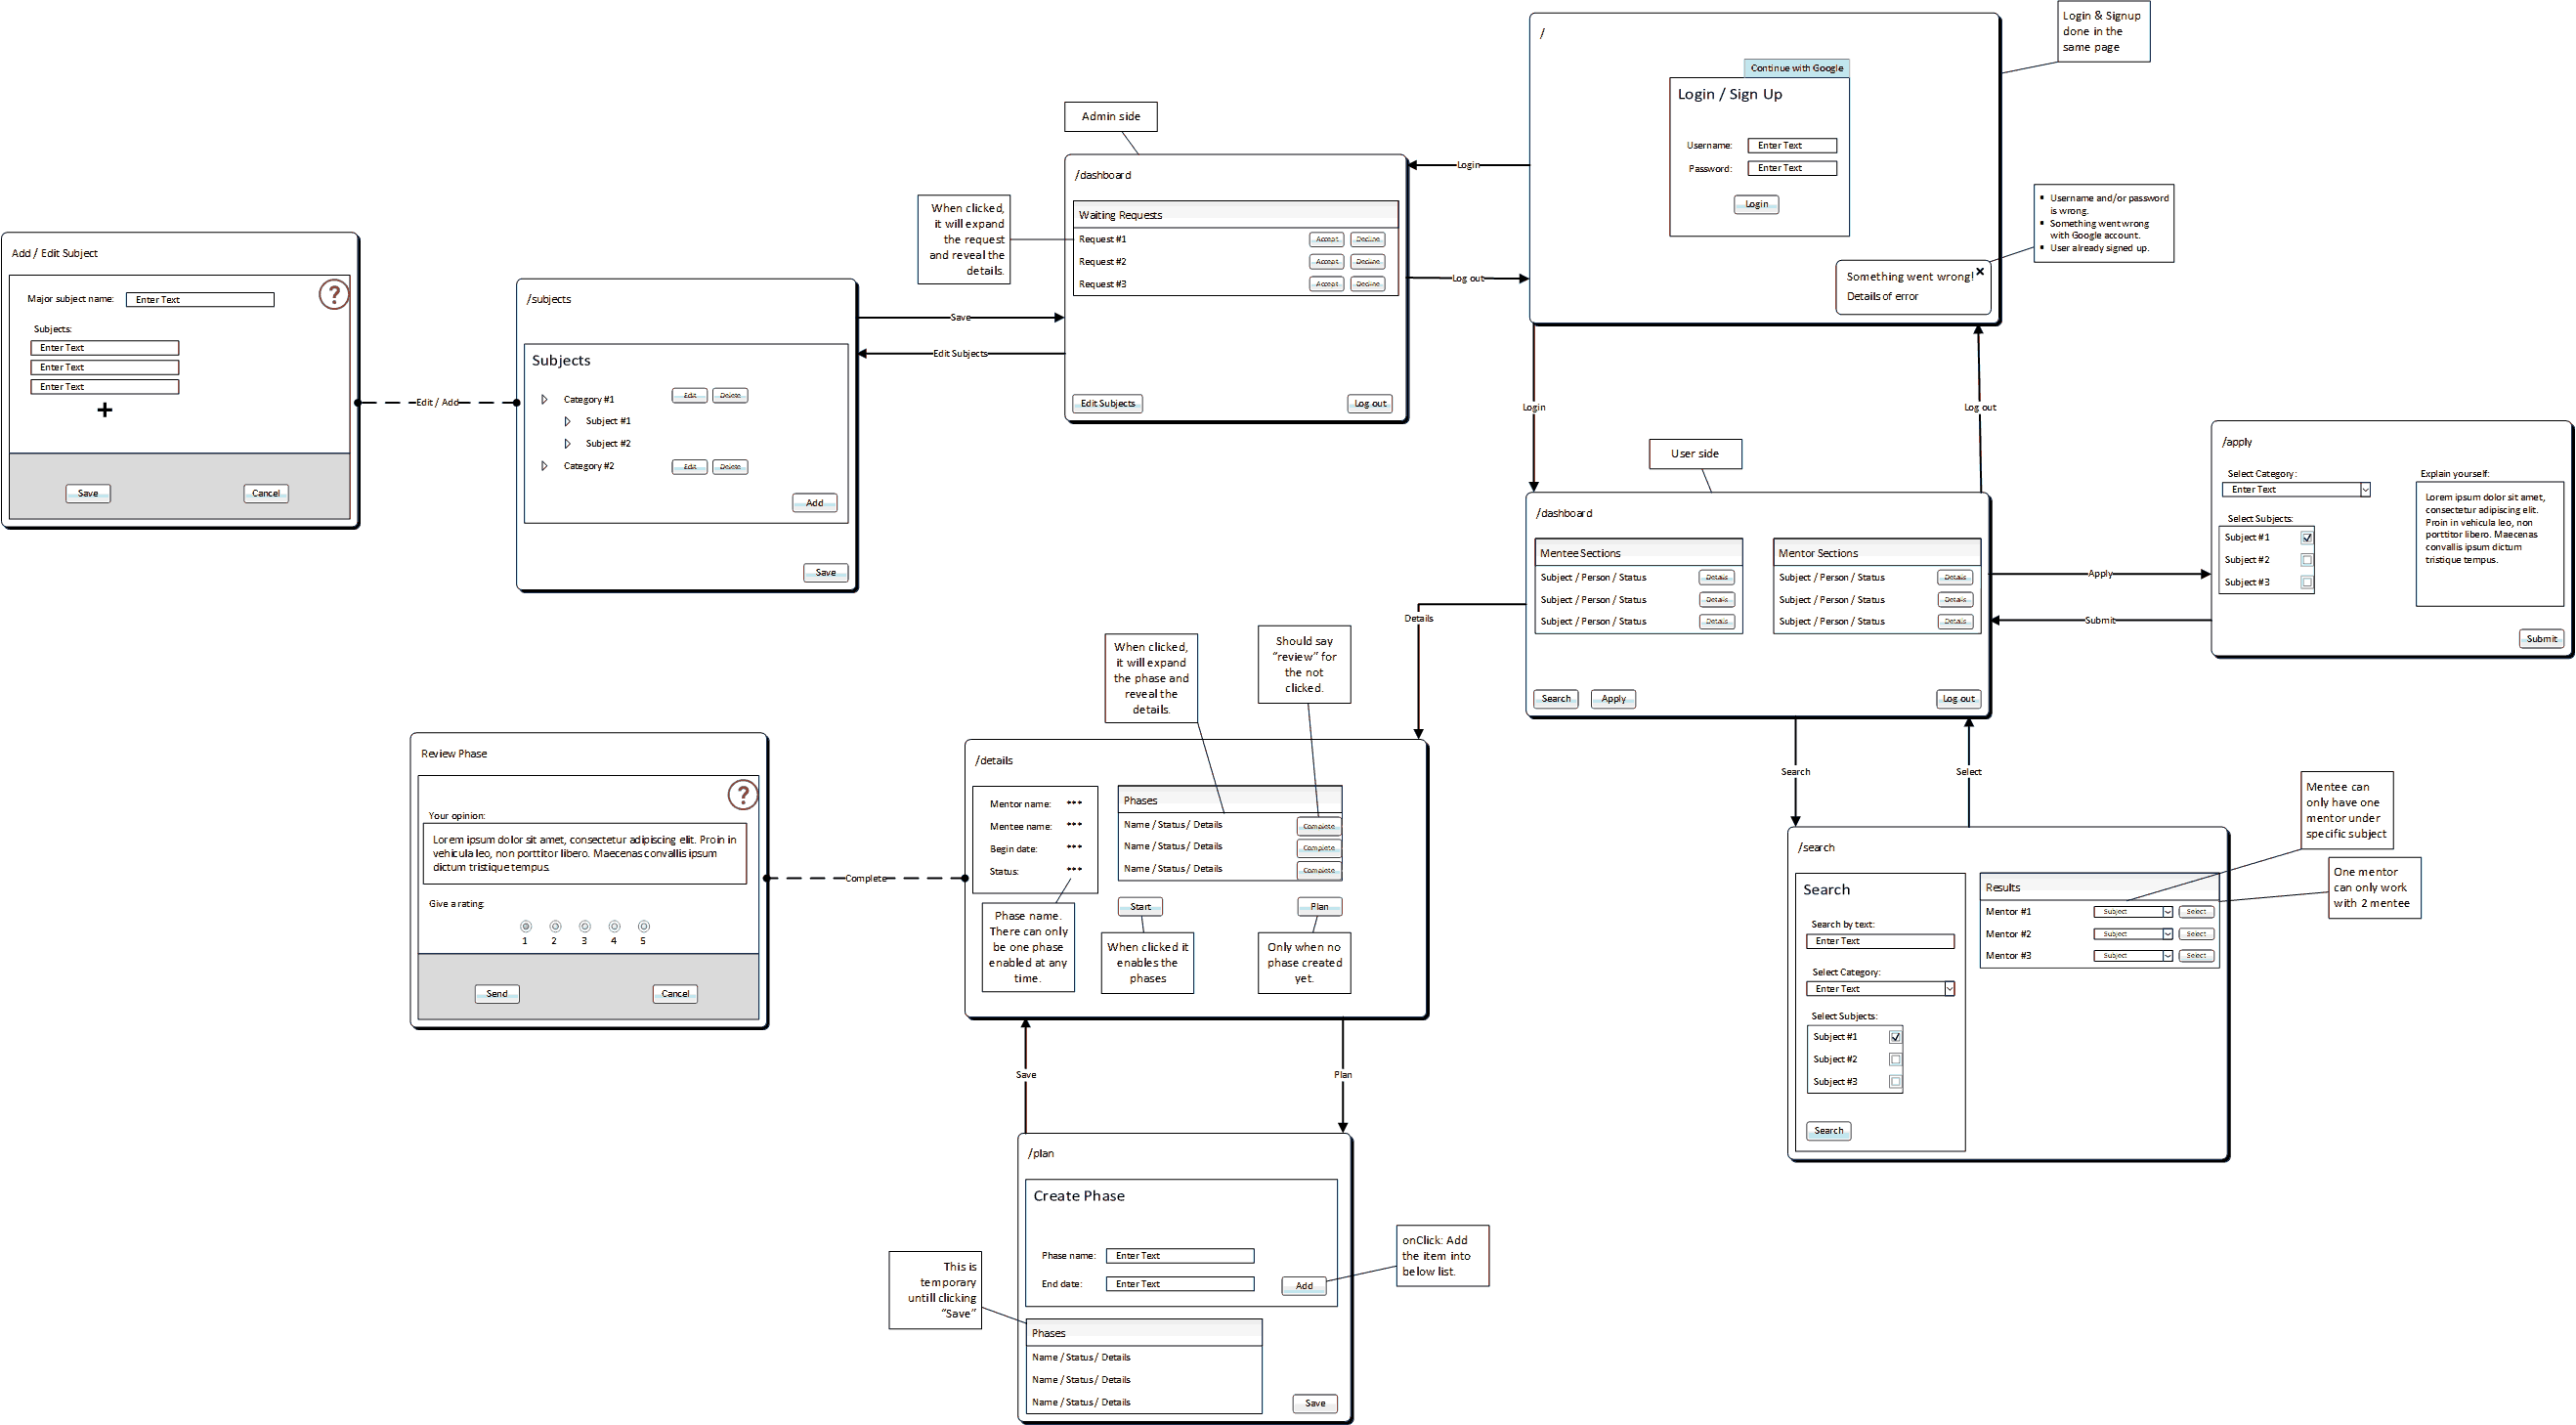
\includegraphics[width=\paperwidth, angle=270]{diagram-views.png}
    \caption{Process flow diagram}
    \label{fig:views}
\end{figure}
\newpage


\subsection{Data Requirements} \label{data_requirements}


\subsubsection{Data Model} \label{data_models}
The data model designed as shown in the below figure \ref{fig:domains}.

\begin{figure}[ht!]
    \centering
    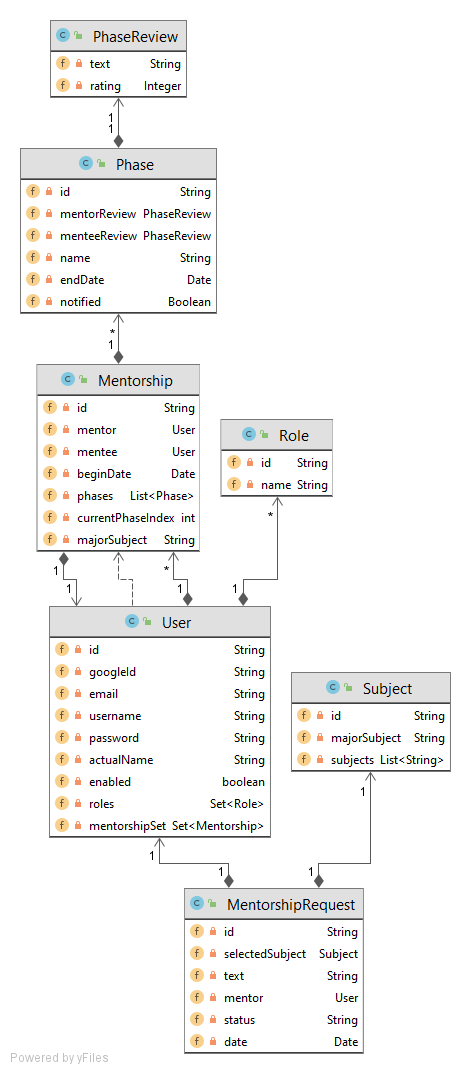
\includegraphics[width=\textwidth]{diagram-domains.png}
    \caption{Entity relationships diagram}
    \label{fig:domains}
\end{figure}

In database, only the classes with \texttt{id} field which is auto--generated by the 
database, have their own collections/tables. Instances of these classes stored as is,
in database.

However, if a field references an entity which is already in the database; for example,
\texttt{mentor} field for \texttt{Mentorship} entity (references to the \texttt{User}
entity), is stored as reference (\texttt{DBRef} for MongoDB) inside the database. 
Otherwise they are stored as embedded documents, such as \texttt{PhaseReview} objects
inside the \texttt{Phase} entities.

In practice the framework will solve this abstraction but know that they are stored
differently in database.
\newpage


\subsubsection{Data Access Mechanism} \label{data_access_mechanism}
Data access done by API calls. The API endpoints are as follows:
\begin{table}[h]
    \centering
    \begin{tabularx}{\textwidth}{|l|l|X|} \hline
        \textbf{Endpoint} & \textbf{Method} & \textbf{Description} \\ \hline
        \texttt{/api/subjects/} & \texttt{PUT} & Creates a new subject or update the existing subject.\\ \hline
        \texttt{/api/subjects/\{idd\}} & \texttt{DELETE} & Remove existing subject.\\ \hline
        \texttt{/api/search/method/text?searchTxt} & \texttt{GET} & Retrieve mentors by full--text search.\\ \hline
        \makecell[l]{\texttt{/api/search/method/filter?} \\ \quad\texttt{majorSubjectName\&subjectList}} & \texttt{GET} & Retrieve mentors by filtering by subjects.\\ \hline
        \texttt{/api/requests/} & \texttt{PUT} & Create mentorship request.\\ \hline
        \texttt{/api/requests/\{id\}/\{answer\}} & \texttt{POST} & Accept or decline mentorship requests.\\ \hline
        \texttt{/api/mentorships/} & \texttt{PUT} & Create mentoring process.\\ \hline
        \texttt{/api/mentorships/\{id\}/phases/} & \texttt{PUT} & Creates a new phase or update the existing phase for mentoring process with \texttt{id}.\\ \hline
        \texttt{/api/mentorships/{id}/nextPhase} & \texttt{POST} & Start the next phase in a mentoring process.\\ \hline
        \makecell[l]{\texttt{/api/mentorships/\{mentorshipId\}/} \\ \quad\texttt{phases/\{phaseId\}}} & \texttt{DELETE} & Remove the phase from mentoring process.\\ \hline
        \makecell[l]{\texttt{/api/mentorships/\{mentorshipId\}/} \\ \quad\texttt{phases/\{phaseId\}/reviews/}} & \texttt{PUT} & Create a review for phase.\\ \hline
    \end{tabularx}
    % \caption{Caption}
    \label{tab:apis}
\end{table}

Only data changes handled by the endpoints. Retrieval of data such as subjects,
user and mentorship details, reviews or phases etc. remained inside the application context.
They are not explicitly shared, they are rendered on the page. This is mainly because to restrict
unwanted access to API endpoints.


\subsubsection{Search Implementation}
As previously explained, actual data stored inside MongoDB. In order to abstract search layer,
Monstache container used. Basically, the purpose of this container is to synchronize the
mentorship request part of the data with Elasticsearch database. So that, the search can be
done with Elasticsearch.

In implementation of the feature, application only needs to know the address of the Elasticsearch
instance. Searching is handled by a dependency of Spring framework. Importing thing is that the
result of the search query is the ids of the relative mentorship requests, converted into
\texttt{SearchHitResponse} class. Then, it needs to be fetched from the database in order to get
additional information. Since the \texttt{id} field is indexed in MongoDB it does not burden the
system.

The separation of database and search engine is due to in future patches, which may
result in a database migration, search feature of the design will not be affected 
(i.e. only the "connector" configuration will be changed).
\newpage


\subsection{Deployment} \label{deployment}
Project can be deployed as Docker image or standalone service. In Docker image all necessary
services and configurations stacked together. Of course, according to necessity each container
can be separated. Such Docker deployment diagram can be seen from the below figure
\ref{fig:deployment}.

\begin{figure}[ht!]
    \centering
    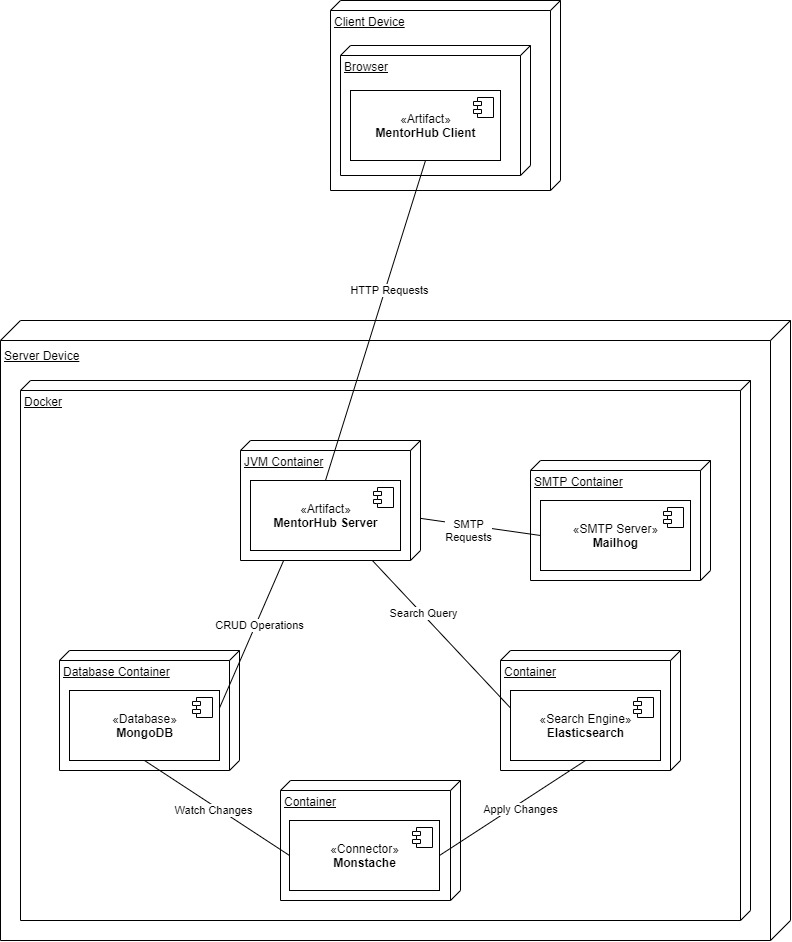
\includegraphics[width=0.95\textwidth]{diagram-deployment.jpg}
    \caption{Physical deployment diagram}
    \label{fig:deployment}
\end{figure}

In development, the program has two main branches: \texttt{master} and \texttt{docker-release}.
\texttt{master} branch mainly used for separated development environment for easier debugging 
and the changes made here (the patches) are applied to \texttt{docker-release} branch. 

So, in order to release product select \texttt{docker-release} branch, compile a JAR file, copy
it to \texttt{<project\_dir>/docker/mentorhub-app/app.jar} and run \texttt{docker-compose up}
command.


\end{document}
